%!TEX root = ../report.tex

% 
% Related work
% 
% (~17pgs)
\section{Related Work}

% começar por dizer como é que está organizada esta secção do trabalho e resumir de uma forma muito geral o que se fala em cada subsecção

This section presents the related work and characterizes the main contributions of past works and how these contributions helped in the development of this project. This section is organized in three main parts: mHealth, mobile security mechanisms and TrustZone.

The first part focuses on describing the attack surfaces of mHealth apps, the most common threats and their seriousness, present a few publicly available insecure mHealth apps as well as some compliance recommendations app developers should follow to avoid unnecessary security risks when handling sensitive health information. The second part of this sections describes the state-of-the-art of mobile security with a particular focus on the Android Operating System and how developers can build secure applications with a trusting \ac{OS} and security mechanisms built upon the application layer. The third part of the related work describes TrustZone, a hardware technology available in most modern \ac{ARM} processors which supports execution of two isolated worlds, a hardware-protected secure world and a normal world. Besides describing the technology, this sections also presents previous work developed using TrustZone and how these contributions may be helpful in achieving the main goals of this project. 

\subsection{mHealth}
\label{sec:mhealth}

As discussed above, mobile devices are increasing in number at astonishing rates, and with this growth the mobile market becomes cheap and accessible. This motivates the shift from mainframe systems, located in the facilities of healthcare providers, to apps on mobile devices as well as storage in shared cloud services. This accessibility also motivates the private sector in building more healthcare applications to support both patients and professionals. Thus, the mobile health market is becoming a competitive market and one which is increasingly handling more sensitive data.

% THREAT TAXONOMY
Kotz, David \cite{kotz2011threat} defines a threat taxonomy for mHealth. In this paper the author categorizes threats in three main categories: \emph{Identity Threats}, \emph{Access Threats} and \emph{Disclosure Threats}.

Identity threats are described as mis-use of patient identities and include cases where a patient may lose (or share) their identity credentials, allowing malicious agents to access their respective \ac{PHR}. \emph{Insiders} (authorized \ac{PHR} users, staff of the \ac{PHR} organization or staff of other mHealth support systems) may also use patient identities for medical fraud or for medical identity theft, and \emph{outsiders} may be able to observe patient identity or location from communications.

Access threats are described as unauthorized access to \ac{PHR} and include cases where the patient, which controls the data, may allow broader-than-intended access or disclosure of information, \emph{insiders} who may snoop or modify patient data with intents other than improving the healthcare of the patient, and even \emph{outsiders} which, by breaking into patient records, may leak or modify this data.

Disclosure threats include cases where an adversary captures network packets in order to obtain sensitive health data, this problem can be mitigated by using strong encryption methods. But even if the network traffic is encrypted it is possible to analyse the traffic to determine its characteristics \cite{wright2006inferring}. The adversary may also use physical-layer, or link-layer fingerprinting, methods to identify the device type and, because the wireless medium is open, an active adversary may inject frames or may selectively interfere with (cause collisions with) wireless frames. These methods may enable the adversary to create a man-in-the-middle situation, to use link-layer fingerprinting methods, or to compromise the devices in a way that divulges their secrets.

This work by Kotz, David \cite{kotz2011threat} helped in understanding what threats are inherent to mHealth systems and their development. An explicit set of rules for developing privacy-sensitive health applications was still needed to ease the development process. Avancha, Baxi and Kotz \cite{avancha2012privacy} filled in the gap by surveying the literature, developing a privacy framework for mHealth and discussing the technologies that could support privacy-sensitive mHealth systems.

% PRIVACY FRAMEWORK FOR MHEALTH

This survey considers essential accounting for privacy in the design and implementation of any mHealth system, given the sensitivity of the data collected. A developer may use the list of privacy properties provided by this article as a check-list to be considered in any design. Furthermore, a set of questions is left open for researchers to improve the efficiency and effect of these properties. It is also mentioned that privacy challenges identified by this article need to be addressed with urgency, because mHealth devices and systems are being deployed now, and retrofitting privacy protections is far more difficult than building them in from the start.

% SECURITY CONCERNS MHEALTH ANDROID
He, Dongjing, et al. \cite{he2014security} analyse several mHealth applications available in Android's app store contributing to the understanding of security and privacy risk on the Android platform. In this paper, three studies were made with the following goals:

\begin{itemize}
	\item \textbf{Study 1: What are the potential attack surfaces?}
	\item \textbf{Study 2: How widespread is the threat?}
	\item \textbf{Study 3: How serious is the threat?}
\end{itemize}

% AQUI ESTOU A DIZER TBM QUE ESCOLHI A APPLICACAO A FAZER POR CAUSA DESTES NUMEROS
In the first study, 160 apps are analysed to find evidence of security threats. From analysing previous literature \cite{zhou2013identity,naveed2014inside,aviv2012practicality,cai2012practicality,chin2011analyzing,fsecure}, seven attack surfaces are determined to be in need of protection. Those seven attack surfaces are shown in table \ref{tab:attacksurfaces}. The authors also document that the 160 apps studied target two different audiences: 129 (81.65\%) are for patients, 32 (20.25\%) are for healthcare professionals and the remaining 3 (1.90\%) are targeted for both. Most apps targated for patients (60\%) are in the Life Management category followed by apps that manage and synchronize user health information (\ac{PHR} Management), which occupy nearly half (46.88\%) of these apps. These numbers are a good indicator of what data is handled by most commercial mHealth apps available and motivate the choice made to build a \ac{PHR} Management app as demo app for TrubiZone.

A few examples of vulnerable applications are also revealed during this study. Regarding unencrypted information sent over the Internet, Doctor Online \footnote{https://play.google.com/store/apps/details?id=com.airpersons.airpersonsmobilehealth} (patients can talk to doctors online) and Recipes by Ingredients \footnote{https://play.google.com/store/apps/details?id=com.abMobile.recipebyingredient} send unencrypted sensitive information, including the user's email and password, in clear text. With regard to logging sensitive information, the study pinpoints CVS/pharmacy \footnote{https://play.google.com/store/apps/details?id=com.cvs.launchers.cvs}, which logs the prescription refill details from user inputs, including name, email address, store number, and Rx number and also logs user login credentials in a debug log message. A malicious party can use this information to view user profiles and prescription history, which could support medical identity theft. In addition, it is even possible to do online pharmacy shopping with user's stored credit card information.

Further applications are given as example for exposing sensitive data. Noom Weight Loss Coach \footnote{https://play.google.com/store/apps/details?id=com.wsl.noom} reveals user workout history by exposing its Content Providers to external apps, which means any app can access the exposed Content Providers without declaring any permission. Finally, this first study concludes with the example of sleep monitoring apps, such as SnoreClock \footnote{https://play.google.com/store/apps/details?id=de.ralphsapps.snorecontrol} and Sleep Talk Recorder \footnote{https://play.google.com/store/apps/details?id=com.madinsweden.sleeptalk}, which store the sleep records of users as unencrypted audio files on external storage. With read permission for the SD card, as well as internet permission, a malicious app can read a user's sleep recordings and even send them to remote servers.

\begin{table}[t]
	\caption {Description of attack surface (taken from He et al. \cite{he2014security})}
	\label{tab:attacksurfaces}
	\begin{tabular}{|>{\raggedright}p{2cm}|>{\raggedright\arraybackslash}p{10cm}|}
		\hline
		\textbf{Attack Surface}      & \textbf{Description}                                                                                                                    \\ \hline
		Internet            & Sensitive information is sent over the internet with unsecure protocols (e.g. HTTP), misconfigured HTTPS, etc.                 \\ \hline
		Third Party         & Sensitive information is stored in third party servers                                                                         \\ \hline
		Bluetooth           & Sensitive information collected by Bluetooth-enabled health devices can be sniffed or injected                                 \\ \hline
		Logging             & Sensitive information is put into system logs where it is not secured                                                          \\ \hline
		SD Card Storage     & Sensitive information is stored as unencrypted files on SD card, publicly accessible by any other app                          \\ \hline
		Exported Components &  Android app components, intended to be private, are set as exported, making them accessible by other apps                     \\ \hline
		Side Channel        & Sensitive information can be inferred by a malicious app with side channels, e.g. network package size, sequence, timing, etc. \\ \hline
	\end{tabular}
\end{table}

In the second study, 27 of the top 1080 free apps from the Medical and Health \& Fitness categories on Google Play were analysed according to their vulnerabilities. From this analysis, three attack surfaces are identified as the most important ones: \emph{Internet}, \emph{Third Party Services} and \emph{Logging}. Only 7 of these 27 apps use the Internet to effectively send medical information over to remote servers. It is important to understand if the information sent over the Internet is protected. To achieve this, the authors captured network traffic and concluded that only 57.1\% (4/7) of these apps use encrypted communication and the remaining 42.9\% (3/7) send unencrypted sensitive health information. Among the unencrypted contents sent by these 3 apps are emails, usernames and passwords. This study also concludes that 85.7\% (6/7) of these apps are hosted and store the recorded data on third party servers. This is an economical and scalable solution for mobile applications, but storing sensitive health records on third party servers can have serious implications, mostly due to app users not being aware that their data is being stored on third party servers and because these users are incapable of telling if this data is stored encrypted in such a way that hosting companies do not have access to it.

Some health apps use Bluetooth devices to collect personal health information such as heart rate, respiration, pulse oximetry, electrocardiogram (ECG), blood pressure, body weight, body temperature, quality of sleep and exercise activities. Naveed et al. \cite{naveed2014inside} show how a malicious app can stealthily collect user data from an Android device or spoof it and inject fake data into the original device's app, in what is called an \ac{DMB} attack. One of the 27 apps analysed in this study connects to external health sensors and uses default PIN code 0000, which makes it vulnerable to the \ac{DMB} attack.

Along with the logging, external storage, exported components and other problems discussed above, which represent explicit channels used for attacks, side channels can be exploited by a malicious party to infer sensitive information from apps, even when they are well-designed and implemented. This study mentions an example by Zhou et al. \cite{zhou2013identity} where a correlation between network payload size and the disease condition a user selects on WebMD mobile \footnote{https://play.google.com/store/apps/details?id=com.webmd.android}. Network payload size is publicly accessible in Android, which represents a problem when such correlations can be made. Zhou et al. \cite{zhou2013identity} mitigate the problem by modifying the Android kernel to enforce limitations on accessing Android's public resources. 

In the third study, another 22 apps, which send information over the Internet, are randomly selected from the same top 1080 apps and audit to understand what information is effectively being sent over the Internet, thus inferring the seriousness of the threats. The conclusion is that, when used as intended, these apps gather, store and transmit a variety of sensitive user data, which includes at least personal profiles, health sensor data, lifestyle data, medical information browsing history and third-party app data (e.g. Facebook account information). Figure \ref{fig:sensitivedistribution} shows the distribution of sensitive data in those 22 apps. Consequences of data breaches, information disclosure or tempering with sensitive health data depend on the type, sensitivity and volume of data breached, but it is clear that profiling, medical identity theft and healthcare decision-making errors are all possible. This is why the authors suggest the use of encryption for communication and storage, and encourage developers to create a set of standard security and privacy guidelines that offer a baseline for protection.

\begin{figure}[t!]
  \centering
  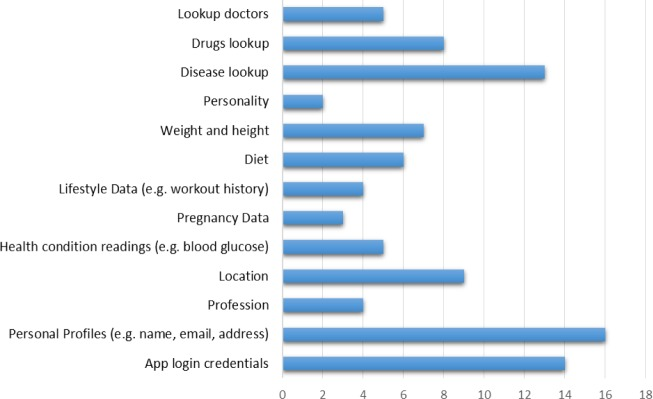
\includegraphics[width=0.95\textwidth]{img/sensitivedistribution.jpg}
  \caption{Sensitive information distribution for study 3 (taken from  He et al. \cite{he2014security})}
  \label{fig:sensitivedistribution}
\end{figure}
%\FloatBarrier

% EM QUE O TRABALHO ME AJUDOU
The work by He, Dongjing, et al. \cite{he2014security} helped in understanding what are the most common attack surfaces when considering mHealth applications on Android and it also helped assessing the security risks inherent to applications handling privacy-sensitive information. This paper generally describes the state-of-the-art of security in commercial mobile health apps and pinpoints what should be fixed in order to build better and more secure application for the healthcare industry. It is clear that developers focus much more on building feature-full applications rather than secure apps and this is why it is important to build a framework which allows developers to completely focus on the features they want to provide without having to focus heavily on security. % We believe that building a developer framework over ARM's TrustZone technology is a good solution because with TrustZone is possible to fully enjoy the potential of the hardware already available in most mobile devices. This technology will be described in section \ref{sec:trustzone}. 

\subsection{Mobile Security Mechanisms}

This section describes the security mechanisms available for the Android platform, either from native Android or as security extensions, and how these mechanisms can be used to solve some of the problems covered in the previous section. Work by Duarte, Nuno \cite{nunoduarte} and Costa, Miguel \cite{miguelcosta} extensively describe Android's security mechanisms and divide them in seven groups: \emph{(i)} digital rights management, \emph{(ii)} access control mechanisms, \emph{(iii)} permission refinement, \emph{(iv)} application communication monitoring, \emph{(v)} privacy enhancement systems, \emph{(vi)} access control hook APIs, and \emph{(vii)} memory instrumentation. Although some of theses systems may not be suited for the needs of the problem we intend to solve, this section aims to be a description of the state-of-the-art regarding security on the Android platform. Moreover, to the seven groups described, we suggest the addition of a new mechanism: \emph{(viii)} embedded security systems. This mechanism is not directly related to Android but, with a significant presence in most modern smartphones, its discussion is imperative for the project.%as well as \textbf{MORE REFERENCES HERE}, which are good sources for information on this section of related work.

\subsubsection{Digital Rights Management}
The first security mechanism analysed is Digital Rights Management. This specific access control technology allows data owners to restrict if and how their data is copied and also how that data is handled once transferred to another device. The \ac{DRM} ecosystem is composed of the following entities:

% estruturar melhor esta lista
\begin{itemize}
	\item \emph{User} - human user of the DRM Content
	\item \emph{Content Issuer} - entity that delivers the content
	\item \emph{Rights Issuer} - entity responsible for assigning permissions and constraints to \ac{DRM} content
	\item \emph{Rights Object} - XML document generated by a Rights Issuer expressing the restrictions associated to the content.
	\item \emph{\ac{DRM} Agent} - trusted entity responsible for enforcing permissions and constraints upon the \ac{DRM} content
\end{itemize}

\ac{DRM} can be used to protect proprietary software, hardware or general content. The most common application for \ac{DRM} nowadays is music and video games, because these represent highly valuable intellectual property. To understand how \ac{DRM} works in the context of mHealth one can suggest a simple example of a \ac{PHR} mobile health application. In this scenario, the healthcare provider (e.g. a hospital) would be the \emph{content issuer}, and it would use a \emph{rights issuer} to assign the restrictions imposed upon the \ac{DRM} content, which in this case would be the personal health record of a patient, when this content is transferred to the patient's device. When using \ac{DRM}, the patient is limited to access the content through a \emph{\ac{DRM} Agent}.

The \ac{OMA} developed a DRM standard \cite{drm} which defines the format of the content delivered to DRM Agents, as well as the way this content can be transferred from the Content Issuer to the DRM Agent. Android provides an extensible DRM framework, called Android DRM Framework \footnote{http://developer.android.com/reference/android/drm/package-summary.html}, allowing application developers to enable their apps to manage rights-protected content by complying with one of the supported DRM schemes (specific mechanisms, enforced by DRM Agents, to handle particular types of files).

This mechanism can be useful for protecting personal healthcare records by restricting the way data can be copied and handled. For this project however, DRM is not enough to ensure the confidentiality, integrity and availability of the sensitive data because it may fail to do so when the operating system is compromised with a malicious agent.

\subsubsection{Access Control Mechanisms}

Access control mechanisms are a security model in which subjects (e.g. user, processes, threads, etc.) can perform actions on the system, namely on resources (e.g. files, sensors, etc.), typically called objects. Android follows a type of access control referenced as \ac{DAC}, heritage from it's Linux based kernel. In a \ac{DAC} system the data owner is responsible for this data and thus determines who can access it. In a Linux system, one can imagine a system administrator creating several files and allowing access to these files, according to certain permissions. In this example, a subject with the specified permissions may access the file like its owner intended. In Android we can think of a similar example, since an application can create and store files in the filesystem, thus becoming the sole owner of these files, it can allow access to these files to any other application.

Although Android inherits the \ac{DAC} from its Linux ancestry, most other resources in Android follow \ac{MAC} policies. In \ac{MAC}, subjects are much more restricted in determining who has access to their resources. An example of this, from the physical security field, are the levels: confidential, secret and top secret. These labels are the only concept available to define the level of clearance of subjects or to classify data. When a subject attempts to access a classified piece of data, a verification is done to assess if this subject's security level matches (or is above) that of the classified piece of data. Similarly, in Android once a subject attempts to access an object, it triggers a policy evaluation by the kernel, which assesses whether the access may be granted. The advantage of this strict system is its robustness, because subjects cannot override or modify the security policy. In Android, applications must specify in their manifests the permissions they require at runtime and after the installation neither applications nor users have any control over the access policies.

Because \ac{MAC} is robust, several systems were created over the years to extend \ac{MAC}'s access control model to other Android resources. SEAndroid \cite{smalley2013security} solves problems related to resources complying with the \ac{DAC} mechanism. The authors ported SELinux \cite{peter2001integrating} to provide \ac{MAC} at the kernel layer. The kernel was then modified to support a new \ac{MAC} policy (e.g., filesystem, IPC) and a new middleware layer (MMAC) was created to extend \ac{MAC} to Android's Binder IPC. TrustDroid \cite{bugiel2011practical} extends the \ac{MAC} mechanism to all the platform's resources (e.g., filesystem which complied with DAC) in order to isolate different domains' sensitive information.

Even though access control mechanisms allow isolation between different subjects in a system, thus enforcing the confidentiality and integrity needed for this project, it still relies on the premise that the underlying middleware and kernel are secure. With this assumption, sensitive data may be at risk when the \ac{TCB} is compromised. For this reason, access control mechanisms are not sufficient to ensure the security needs of this project.  

\subsubsection{Permission Refinement}
\label{sec:permissionrefinement}

The Android permission mechanism is a very restrict system. At install time, a list of permissions an application specifies in its manifest file is shown to the user, which is forced into a binary decision, either granting all permissions or quitting the installation. This is an inflexible solution, which makes it impossible for users to have full control of the permissions an application is effectively using at runtime. This inflexibility allows apps to use the device's resources whenever the app wishes without the user's knowledge, possibly with malicious intent. Moreover, this permission mechanism allows for some problems such as component privilege escalation. An example of this is when an application, which profits from displaying in-app ads, requests access to the camera and to the Internet. In this case, the ad component has access to the camera, which it should not have because there is no need for it, and furthermore the component may even escalate its privileges by leaking video through the Internet.

Over the years many systems solved some of the problems inherent to permission refinement. APEX \cite{nauman2010apex} modified Android's permission model to allow users to specify the assignment of permissions to each app, both at install and runtime. Permission Tracker \cite{kern2012permission} allows users to be informed on how the permissions are used at runtime and offers the possibility of revoking these permissions. Furthermore, a user can specify which permissions are of interest so they can be notified of every permission access and decide whether to grant or deny that access. Compac \cite{wang2014compac} also restrains application access to certain permissions, but does so considering applications as groups of components and preventing component privilege escalation.

These systems improve upon the original Android permission model, but require manual configuration by the user. A more useful solution would be to use a context-aware system to handle the permissions at runtime. This way it may be possible to, without manual configuration, restrict permissions to all applications running along side a security sensitive application, thus isolating this application and avoiding possible leaks by shared resources. Several context-aware permission refinement systems exist. Trusted third parties can use CRePE \cite{conti2011crepe} to enforce security policies on another devices whilst, for example, the employees' mobile devices are inside the company, but have no privileges otherwise. Similarly, MOSES \cite{russello2012moses} enforces domain isolation through the concept of security profiles. MOSES can switch security profiles based on pre-established conditions (e.g., GPS coordinates and time). When switching from a personal (less restrictive) profile to a professional (more restrictive) one, MOSES terminates and prevents the execution of applications not allowed to run in the new enforced profile. Additionally, MOSES leverages TaintDroid \cite{enck2014taintdroid} (covered in Section \ref{sec:privacyenhancement}) to prevent apps from one profile to access data belonging to another.

Both CRePE and MOSES suffer from a device control issue where a third party defines a policy that cannot be revoked by the user. Moreover, a user has no way to deny the enforcement of a third party policy. Duarte \cite{nunoduarte} and Costa \cite{miguelcosta} developed a system called TrUbi, built on top of ASM \cite{heuser2014asm} (covered in Section \ref{sec:accesscontrolhooks}), which solves the problems mentioned and presents a developer friendly framework for the development of sensitive permission refinement applications.

Even though TrUbi could be a good base for the development of this project, by allowing the development of applications which can control and enforce restrictions over less secure-sensitive apps, it suffers from the same limitations as the mechanisms discussed previously. When the underlying middleware and kernel are compromised, the security sensitive data may become accessible by a malicious agent.

\subsubsection{Application Communication Monitoring}
\label{sec:appcommmonitoring}

Another problematic mechanism in Android is the way applications interact with each other. Some problems were already described in section \ref{sec:mhealth} regarding vulnerable mobile health applications, which fall into this category. Two attacks will be described in this section, followed by systems developed to mitigate such attacks on Android. The two attacks described are called \emph{Confused Deputy Attacks} and \emph{Collusion Attacks} and are represented in Figure \ref{fig:communicationattacks}. Confused deputy attacks basically consist of unprivileged applications taking advantage of other applications’ publicly accessible APIs to perform malicious actions. Collusion attacks consist of an app, which might not have permission to perform an operation, still being able to perform it if there exists another app, belonging to the same developer, installed on the user’s device with the permission to perform said operation. This happens because Android’s permission system is based on UIDs.

% será que é mesmo necessário?
Confused deputy attacks allow applications to use resources without explicitly specifying the necessary permission to do so. A simple example is an app that exposes a service on its API allowing another app to receive photos directly from the device's camera. The second app, which did not specify the camera permission, can access this sensor without the user's knowledge. If this second app is malicious and has access to the Internet, then it becomes clear the severity of the problem, which may lead to sensitive information being leaked. This problem generally happens because of poor or negligence application development.

A system  called Saint \cite{ongtang2012semantically} was created to specify which apps can access the public APIs of another app. This is done by allowing developers to assign appropriate security policies on their APIs. The identity of the caller apps is authenticated by the modified \ac{IPC} mechanism. Other systems control this communication by extending Android’s Binder \ac{IPC} mechanism, which is the main form of application inter-communication in Android. QUIRE \cite{dietz2011quire} denies access to an API if in the message exchanged between apps, which contains the full call chain context, the source of the request does not have the necessary permission to access the corresponding data.

% será que é mesmo necessário?
Collusion attacks are based on a malicious developer building a legitimate application with permissions such as microphone access and persuading the user to install another app with Internet permission. Both apps can collude to leak sensitive audio data through the Internet because Android's permission system is based on UIDs, thus, although the first app does not explicitly request Internet access, this resource is accessible because the developer has Internet access through the second app.

XManDroid \cite{bugiel2011xmandroid} extends the Android permission model in order to support policies that could constrain the way apps interact with each other. This system prevents data leakage or other types of collusion attacks by developing a graph at runtime with a representation of the apps’ interactions, which is then used to regulate app inter-communication.

\begin{figure}[t!]
	\centering
	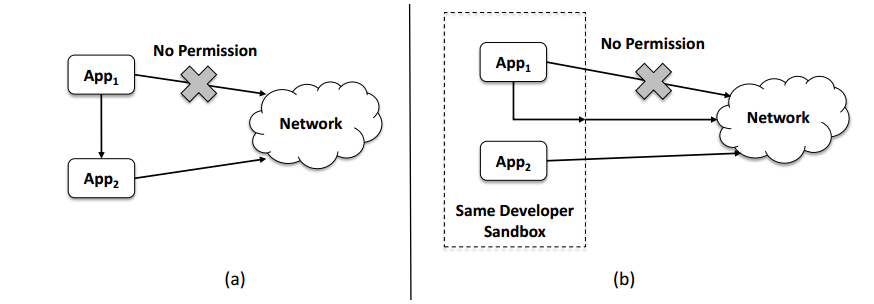
\includegraphics[width=0.95\textwidth]{img/communicationattacks.png}
	\caption{Confused deputy attack (a); Collusion attack (b) - (taken from Duarte \cite{nunoduarte})}
	\label{fig:communicationattacks}
\end{figure}

% REVER ISTO
Although these systems assist the development of more secure mobile applications on the Android platform, by themselves these systems are not capable of building security sensitive apps and thus are not suitable for this project.

\subsubsection{Privacy Enhancement Systems}
\label{sec:privacyenhancement}

The most important concern for a privacy-sensitive mobile application is the way data is managed, specially with valuable data such as health records or banking information. Many systems have been developed to target different privacy problems in the Android environment.

%rever isto, está muito copiado?
%TODO
Systems like MockDroid \cite{beresford2011mockdroid} and Zhou et al. \cite{zhou2011taming} are extensions to Android's data access control and prevent untrusted applications from accessing sensitive data by allowing users to manually specify application access rights over the system services. These systems even offer data shadowing \footnote{Data shadow is the return of empty or incorrect information instead of the intended data.} to the unauthorized apps trying to access it. Other systems, like IdentiDroid \cite{shebaro2014identidroid} focus on protecting the identity of the user. This is done by using an anonymous mobile device state to provide data shadowing and permission revocation techniques that disable the ability of apps to use systems services such as location or \ac{IMEI}. This way if an app is trying to use the devices location, a default location is returned instead of the real one or the application simply cannot access the location service.

Some systems use a different approach to solve the same problem. Dynamic taint analysis systems prevent data leakage by tainting data with a specific mark and then evaluate how this data is propagated through the system. If this data attempts to leave the system the user is alerted. TaintDroid \cite{enck2014taintdroid} does this by modifying Android's Dalvik VM environment and Binder \ac{IPC} to track the information within different applications' processes. Although TaintDroid is an interesting system, it suffers from limitations which include: \emph{(i)} tracking a low number of data sources (mainly sensors), \emph{(ii)} performance overheads not tolerable for most mobile environments, \emph{(iii)} the existence of false positives leading to access control circumvention and \emph{(iV)} the incapacity of analysing sensitive information leakage through covert channels.

% será mesmo necessário?
Despite these limitations, TaintDroid was used by the research community as a building block for other privacy enhancement systems. Kynoid \cite{schreckling2013kynoid} extends TaintDroid to support a bigger number of information sources and to provide users a way to establish data access rights on data items and allows the to specify a list of acceptable IP destinations for each item. Another TaintDroid based system is AppFence \cite{hornyack2011these}, which provides a mechanism to block data made available by the user for on-device use only to be transmitted over the network, and allows for high level data to be substituted by shadowed data.

Although these systems aim at protecting users' privacy they focus on detecting and preventing data leakage instead of providing a framework for developers to build privacy-sensitive applications. Even if a good framework for privacy-sensitive app development existed the limitation discussed before would still persist. If the middleware or kernel layers become compromised then all systems dependent of these will be compromised as well.

\subsubsection{Access Control Hook APIs}
\label{sec:accesscontrolhooks}

A trend from previous work on mobile security is clearly noticeable: most security extensions require modifying and adding components to the kernel and middleware layers in order to implement new security models. Some frameworks have been built to ease the development process by allowing developers to easily create security models as ordinary apps whilst benefiting from a full callback system capable of notifying the security enforcement applications of accesses and requests to some of the apps' resources of interest.

These frameworks comprise a set of hooks distributed among the kernel and middleware layers, which can be registered by a secure application. When a hook is activated it triggers a callback from the Hook API module, which in turn is forwarded to the app for verification. The app then decides if the operation that triggered the activation of the hook may or may not proceed. The main advantage of frameworks such as \ac{ASM} \cite{heuser2014asm} and \ac{ASF} \cite{backes2014android} is the flexibility and freedom given to developers in choosing whatever resources to manage.

TrUbi \cite{miguelcosta,nunoduarte} is built upon ASM and allows for flexible system-wide resource restriction, which may be used to isolate privacy-sensitive apps by killing, freezing or revoking permissions to running applications. The limitation of TrUbi is already discussed in section \ref{sec:permissionrefinement} and is based upon the fact that the \ac{TCB} is comprised of all the Android kernel, Android middleware and extensions such as \ac{ASM}.

\subsubsection{Memory Instrumentation}
\label{sec:meminstrumentation}

Memory instrumentation can be divided in two groups: static memory instrumentation and dynamic memory instrumentation. While static memory instrumentation changes already compiled bytecode, dynamic instrumentation patches running processes. In the remainder of this section the sole focus will be on dynamic memory instrumentation as it is an interesting mechanism to enforce new security models.

DeepDroid \cite{wang2015deepdroid} relies on dynamic memory instrumentation to enforce fine-grained context-aware security policies for enterprise. This is done by patching several system services and tracing system calls. But this system is better suited for the development of new security policies instead of suiting the development of robust privacy-sensitive applications like the one we intend to build.

Therefore, this security mechanism is not adequate for the needs of this project. Moreover, these systems still suffer from the same limitations discussed previously regarding compromised operating systems and large trusted computing bases. 

\subsubsection{Embedded Security Systems}

Although developing new security mechanisms for mobile platforms like Android and iOS is important, mobile security is not limited to secure software. This section describes the embedded security architectures available on the market, along with its strengths and weaknesses. A whitepaper \cite{trustzone_whitepaper} by \ac{ARM} states that security solutions for embedded applications fall into four categories, which will be explained in the remainder of this section.\\

\textbf{External hardware security modules} represent the classic security solution for embedded applications, which is the inclusion of a dedicated trusted element (e.g., a smartcard) that is outside of the main \ac{SoC}. On one hand, the main advantage of this solution is that it allows for the encapsulation of sensitive assets inside a physical device specially designed for robust security. On the other hand, the main disadvantage is that smartcards provide only secure processing and storage functions. This means that some operations (e.g., I/O) must rely on software running outside of the security perimeter to provide the desired features. An example where this happens is when a user interacts with the system by entering a \ac{PIN}. This \ac{PIN} must be managed by the less secure software outside of the smartcard, making it vulnerable to attacks.\\

%rever, muito copiado
\textbf{Internal hardware security modules} are, contrary to the previous solution, included within the \ac{SoC}. These integrated modules are usually one of two forms: the first is a hardware block designed specifically for managing cryptographic operations and key storage, and the second is a general purpose processing engine, which is placed alongside the main processor, that uses custom hardware logic to prevent unauthorized access to sensitive resources.

This solution has the advantage of being cheaper and offering a performance improvement over external hardware security modules like smartcards. The disadvantage is that, like the previous solution, the resources protected by the security module will eventually need to be used outside the module it self, thus making these resources vulnerable. Another disadvantage is that this design requires a separate physical processor, typically less powerful than the main processor, to a avoid sharing such an important resource with less critical modules. Extending or migrating systems built with this solution is also much harder, because separation of resources must be implemented on proprietary hardware extensions within the \ac{SoC}.\\

\textbf{Software virtualization} is another security mechanism which has been growing in popularity over the past years. In this software security mechanism, a highly trusted management layer called hypervisor runs in a privileged mode of a general purpose processor. The hypervisor uses a \ac{MMU} to separate several independent software platforms, running each one inside a virtual machine.

There are many advantages of using this solution. The first advantage is that a compact hypervisor can be thoroughly tested to ensure, with a high degree of certainty, that software running within one virtual machine cannot influence and attack the execution of others running in parallel. Another advantage is that there is no additional hardware requirement to implement a hypervisor, thus any processor with a \ac{MMU} can be used to implement this security solution. Lastly, this solution is capable of supporting processing isolation between a secure environment and a full-blown rich operating system running in different virtual machines managed by the hypervisor. If a communication mechanisms is supported by the hypervisor, then a secure pipeline can be established between the two virtual machines.

The main problem with this approach is the isolation provided is restricted to the processor implementing the hypervisor. If all the other resources, mainly system buses, are not managed by the hypervisor, then the protection provided by the virtualization may be bypassed. Managing resources, like \ac{GPUs}, can be difficult to achieve without hindering the system's performance.\\

\textbf{TrustZone} is a hardware architecture that extends the security throughout the system design. TrustZone's architecture was designed to mitigate the problems discussed above. This is achieved by allowing any part of the system to be made secure, instead of protecting only the assets inside a secure hardware block, thus enabling end-to-end security without exposing resources to a less critical platform.\\

To accomplish the goals of this project, a completely secure flow of execution is needed, this means that privacy-sensitive data must never leave the trusted security perimeter. A system which does not support secure I/O greatly limits the functionality offered by a \ac{PHR} application, to the point where it becomes useless. For this reason we exclude both the external and internal hardware security modules as viable solutions for the problem.

On a different note, the virtualization solution seems promising, but with all the problems related to sharing resources such as \ac{GPUs} and other system buses, this security module can be discarded as a solution. For an application to be secure, even when the rich OS is compromised, total isolation is needed, which is not easily achievable using virtualization by it self.

TrustZone technology seems to be the most complete system of all the embedded solutions, as it mitigates recurring problems from other mechanisms. Considering this, TrustZone is the most viable solution for our \ac{PHR} application, because it allows for a complete isolation between the privacy-sensitive data and all the other non-critical logic. 

\subsubsection{Summary}

After describing and assessing the available technology, one can argue which mechanisms better suit the development of critical mobile applications for Android, such as our \ac{PHR} app. Some mechanisms are clearly unsuitable for the goals of this project. Application communication monitoring (section \ref{sec:appcommmonitoring}), access control hook APIs (section \ref{sec:accesscontrolhooks}) or memory instrumentation (section \ref{sec:meminstrumentation}) may be helpful in mitigating vulnerabilities caused by negligent development or for the development of new access control policies respectively, but are not sufficient to build privacy-sensitive applications. A summary of the main conclusions for the remaining systems studied is shown in table \ref{tab:securityMechanismsComparison}.

\ac{DRM} by it self is capable of protecting data from disclosure and modification, hence it would be a great candidate for securing a privacy-sensitive application. Using access control mechanisms is possible to achieve data integrity and non-disclosure of sensitive data by restricting access to critical resources by untrusted applications, for example, by disabling Internet access to all untrusted apps one guarantees that sensitive data will not be leaked using this resource.

With permission refinement systems, in particular with TrUbi, it is possible to isolate the execution of a critical application from the remaining apps installed on the system, for example, the \ac{PHR} app could be developed with the following premise. When the \ac{PHR} app is running, all the other apps are killed and all the resources blocked.The app could then download the health records from the healthcare provider and show the data to the user. When the user exits the application, their data is encrypted with a key generated from a user password, and only then the resources are released for the other applications. The system was completely isolated during the whole process and the data is stored with encryption (and the key, because it is generated from a user password, is not stored on the system).

Although all of the above solutions are suitable for building a secure \ac{PHR} application, they do not achieve the goals of this project, because all of these mechanisms suffer from the same limitation: both the middleware and the underlying kernel are considered as \ac{TCB}. This means that if a malicious app is capable of compromising these layers, then the critical \ac{PHR} application is compromised as well, and the data it protects may be accessible by the malicious party. 

The only solution for the problem described is an hardware based security mechanism. As shown in table \ref{tab:securityMechanismsComparison}, the embedded security technology, particularly TrustZone, is the only solution which works either with a trusted OS and a compromised OS. For this reason, the next section will focus on describing the state-of-the-art, architecture and functionality of TrustZone technology, as it is the only security mechanism suitable for the needs of this project.

% Please add the following required packages to your document preamble:
% \usepackage{graphicx}
\begin{table}[t!]
	\centering
	\caption{Comparison between security mechanisms with and without a compromised Operating System (Android).}
	\label{tab:securityMechanismsComparison}
	\resizebox{\textwidth}{!}{%
		\begin{tabular}{|l||l|l|l|l|}
			\hline
			\multirow{2}{*}{Security Mechanism} & \multicolumn{2}{c|}{Trusted OS}  & \multicolumn{2}{c|}{Compromised OS} \\ \cline{2-5}
			                                    & Confidentiality & Data Integrity & Confidentiality & Data Integrity    \\ \hline \hline
			Digital Rights Management           & \cmark          & \cmark         & \xmark          & \xmark            \\ \hline
			Access Control Mechanisms           & \cmark          & \cmark         & \xmark          & \xmark            \\ \hline
			Permission Refinement               & \cmark          & \cmark         & \xmark          & \xmark            \\ \hline
			Privacy Enhancement Systems         & \cmark          & \cmark         & \xmark          & \xmark            \\ \hline
			Embedded Security Technology        & \cmark          & \cmark         & \cmark          & \cmark            \\ \hline
		\end{tabular}
	}
\end{table}

% TRUSTZONE
\subsection{TrustZone}
\label{sec:trustzone}

O QUE É A TRUSTZONE\\
A ARQUITECTURA DA TRUSTZONE\\
O TRABALHO PREVIAMENTE EFECTUADO COM TRUSTZONE (COM E SEM A PLACA)




